\section{Fibrant Cubesets and Their Weak Structure Theory}
This section deals with the weak structure theory of cubesets.
First, we discuss the notion of a fibration. Then, we consider truncated cubesets and their homotopy groups.
Using this, we obtain the structure tower of a concrete fibrant cubeset, which is studied in the last subsection.

\subsection{Fibrations}\label{ssec:fibrations}


In this section we work in the unrestricted (classical) category of cubes $\bbox$
with all morphisms (projections, permutations and flips).

Recall that given $n\in\N$ there are $n$ many canonical inert maps $\epsilon^{n-1}_i\colon\langle n\rangle\to\langle n-1\rangle$ in $\fin_\ast$ which are
the unique monotonic surjections being undefined in $i$, i.e. given by $j\mapsto j$ if $j<i$, $i\mapsto\ast$ and $j\mapsto j-1$ if $j>i$.
We denote the corresponding maps in $\bbox$ by $\epsilon_i^{n-1}$
(or simply $\epsilon_i$ if the dimension $n$ is clear from the context) as well,
which now correspond to lower face maps and are inclusions ${\bbox}^{n-1}\to{\bbox}^n$.
The image of $\epsilon_i^{n-1}$ is the subset $[x_i = 0] = \{x\in\{0,1\}^n : x_i = 0\}$ for $1\leq i\leq n$.

\begin{definition}\label{def:corner}
Let $n\geq 1$.
The $n$-corner ${\bbcor}^n$ of the $n$-cube ${\bbox}^n$ is the union of all $(n-1)$-cubes ${\bbox}^{n-1}\subset{\bbox}^n$ such that the inclusion arises from an inert map in $\fin_\ast$.

Equivalently, it is the colimit over the diagram of all representable subobjects
${\bbox}^m\sub{\bbox}^n$ for $m<n$ such that the inclusion is inert,
meaning that it is a composition of maps of the form $\epsilon_i$.
\end{definition}

\begin{center}

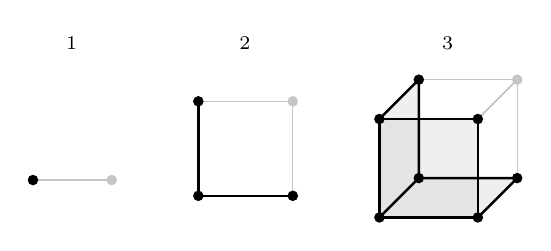
\begin{tikzpicture}[
    x=1cm,y=1cm,
    font=\small,
    line cap=round,
    line join=round,
    vertex/.style={circle,fill,inner sep=1.35pt},
    greyvertex/.style={circle,fill=gray!45,inner sep=1.35pt},
    ambient/.style={draw=gray!45,line width=0.45pt},
    corneredge/.style={draw=black,line width=0.9pt},
    cornerface/.style={
        draw=gray!55,
        fill=gray!45,
        line width=0.45pt,
        fill opacity=0.28
    },
    toplabel/.style={font=\normalsize},
scale=0.5
]

\node[toplabel] at (1.0,3.35) {$\bbcor^1$};
\node[toplabel] at (5.4,3.35) {$\bbcor^2$};
\node[toplabel] at (10.55,3.35) {$\bbcor^3$};

\begin{scope}[shift={(0,0)}]
    \coordinate (A) at (0,0);
    \coordinate (B) at (2,0);

    \draw[ambient] (A)--(B);

    \node[vertex] at (A) {};
    \node[greyvertex] at (B) {};
\end{scope}

\begin{scope}[shift={(4.2,-0.4)}]
    \coordinate (A) at (0,0);
    \coordinate (B) at (2.4,0);
    \coordinate (C) at (0,2.4);
    \coordinate (D) at (2.4,2.4);

    \draw[ambient] (A)--(B)--(D)--(C)--cycle;

    \draw[corneredge] (A)--(B);
    \draw[corneredge] (A)--(C);

    \node[vertex] at (A) {};
    \node[vertex] at (B) {};
    \node[vertex] at (C) {};
    \node[greyvertex] at (D) {};
\end{scope}

\begin{scope}[shift={(8.8,-0.95)}]
    \coordinate (A) at (0,0);
    \coordinate (B) at (2.5,0);
    \coordinate (C) at (0,2.5);
    \coordinate (D) at (2.5,2.5);

    \coordinate (E) at (1.0,1.0);
    \coordinate (F) at (3.5,1.0);
    \coordinate (G) at (1.0,3.5);
    \coordinate (H) at (3.5,3.5);

    \draw[ambient] (A)--(B)--(D)--(C)--cycle;
    \draw[ambient] (E)--(F)--(H)--(G)--cycle;
    \draw[ambient] (A)--(E);
    \draw[ambient] (B)--(F);
    \draw[ambient] (C)--(G);
    \draw[ambient] (D)--(H);

    \filldraw[cornerface] (A)--(B)--(D)--(C)--cycle;
    \filldraw[cornerface] (A)--(B)--(F)--(E)--cycle;
    \filldraw[cornerface] (A)--(C)--(G)--(E)--cycle;

    \draw[corneredge] (A)--(B)--(D)--(C)--cycle;
    \draw[corneredge] (A)--(E)--(F)--(B);
    \draw[corneredge] (E)--(G)--(C);

    \draw[ambient] (D)--(H);
    \draw[ambient] (F)--(H);
    \draw[ambient] (G)--(H);

    \foreach \P in {A,B,C,D,E,F,G}
        \node[vertex] at (\P) {};

    \node[greyvertex] at (H) {};
\end{scope}
\end{tikzpicture}
\end{center}

Note that the point ${\bbox}^0$ doesn't have a corner.

\begin{remark}\label{rem:corner-combinatorial}
An $n$-corner in $X$ is a map $\lambda\colon{\bbcor}^n\to X$, i.e. an element of $\hom({\bbcor}^n,X)$.
Explicitly, it consists of a tuple of maps $\lambda_i\colon{\bbox}^{n-1}\to X$ for $1\leq i\leq n$
such that whenever $\epsilon_j\colon{\bbox}^{n-2}\to{\bbox}^{n-1}$ is an inert map for $1\leq j\leq n-1$
we have that
\[
    \begin{cases}
        \lambda_i\circ\epsilon_j = \lambda_{j+1}\circ\epsilon_i\quad&\text{for}\; i\leq j, \\
        \lambda_i\circ\epsilon_j = \lambda_j\circ\epsilon_{i-1}\quad&\text{for}\; i\geq j+1.
    \end{cases}
\]
\end{remark}

\begin{remark}
The $n$-corner ${\bbcor}^n$ is a compact connected object%
\footnote{In a category $\cC$, an object $X$ is compact if $\hom(X,-)$ preserves filtered colimits,
and it is connected if $\hom(X,-)$ preserves coproducts.}
in $\cSet$,
as it is a finite colimit of tiny (so in particular compact and connected) objects, the $k$-cubes,
over a connected diagram%
\footnote{A connected object in the category of small categories,
equivalently every two objects in the diagram are connected by a zig-zag of morphisms.}.
Explicitly this means that the functor $\hom({\bbcor}^n,-)\colon\cSet\to\set$ preserves filtered colimits and arbitrary coproducts.
\end{remark}

\begin{definition}\label{def:nil-fibration}
We set
\[
    \Lambda = \{{\bbcor}^n\to{\bbox}^n : n\in\N\}
\]
to be the set of all corner inclusions $\lambda^n\colon{\bbcor}^n\to{\bbox}^n$.
Now a map $f\colon X\to Y$ of cubesets is a \emph{fibration}
if it has the right lifting property against $\Lambda$, i.e.,
for every commutative diagram
\begin{center}
\begin{tikzcd}
	{{\bbcor}^n} & X \\
	{{\bbox}^n} & Y
	\arrow[from=1-1, to=1-2]
	\arrow[hook', from=1-1, to=2-1]
	\arrow[from=1-2, to=2-2]
	\arrow[dashed, from=2-1, to=1-2]
	\arrow[from=2-1, to=2-2]
\end{tikzcd}
\end{center}
there exists a diagonal filler.
Moreover, a cubeset $X$ is \emph{fibrant} if the projection $p\colon X\to\ast$ is a fibration.
We denote the full subcategory of fibrant cubesets by $\cSetnil$.
\end{definition}

Geometrically, a fibration is a map $f$ such that every $n$-corner in $X$,
whose image under $f$ comes from an $n$-cube in $Y$, already arose from an $n$-cube in $X$.
We also say that a fibrant cubeset has \emph{corner completion}.

\begin{example}
The $n$-cube ${\bbox}^n$ is not fibrant for $n\geq 1$, but the point ${\bbox}^0=\ast$ is.
For this, consider, e.g. the $2$-corner spanned by twice the same nondegenerate $1$-cube in ${\bbox}^n$.
This does not extend since any affine linear extension to $\bbox^2$ would necessarily map the new vertex to something outside the $n$-cube.

Injective objects such as the subobject classifier $\Omega$, or more generally $\Omega^X=\ihom(X,\Omega)$ are fibrant (see \cite[Chapter IV.10, Corollary 2]{MacLane1994}),
as well as discrete and trivial objects $i_\ast S$ and $i_!S$ for nonempty sets $S$.
The Host-Kra cubegroups from Example \ref{ex:host_kra_cubegroups} are also fibrant.
\end{example}

\begin{remark}
Note that in this definition we do not include right lifting against the map $\emptyset\to\ast$,
which would correspond to the $n=0$ case in \cite[Definition 7.1]{Gutman2020}.
Our convention seems to agree with \cite[Definition 3.3.7, Lemma 3.3.9]{Candela2017} although there is no explicit definition of the index $n$.
This means that a fibration need not be surjective in general, take for example the map $\emptyset\to\ast$ (or any map with empty domain).
However, every fibration between non-empty concrete ergodic (see Section \ref{ssec:connectivity}) cubesets is surjective.
\end{remark}

\begin{remark}
Equivalently, a cubeset $X$ is fibrant if restricting an $n$-cube to its $n$-corner
\[
    \hom({\bbox}^n,X)\to\hom({\bbcor}^n,X)
\]
is a surjection for all $n\in\N$.
If $X$ is concrete, then an $n$-corner $\lambda$ in $X$ is given by a map
\[
    \lambda\colon\{0,1\}^n\setminus\{1^n\}\to X_0
\]
such that the restriction of $\lambda$ along every lower face
$\epsilon_i\colon \{0,1\}^{n-1}\to\{0,1\}^n$ yields an ($n-1$)-cube of $X$,
i.e., an element of $X_{n-1}$.
Thus, being fibrant amounts to finding a value $\lambda(1^n)\in X_0$
such that the extension $\lambda\colon\{0,1\}^n\to X_0$ is in $X_n$.
\end{remark}

Given the notion of fibration it is possible to construct a \emph{weak factorization system}
$(l(r(\Lambda)),r(\Lambda))$ where $r(\Lambda)$ is the class of fibrations
(those maps with the {\textbf{r}ight lifting property} against $\Lambda$)
and $l(r(\Lambda))$ is the class of \emph{trivial cofibrations},
defined to be the class of all maps that have the {\textbf{l}eft lifting property} against all fibrations.
Being a weak factorization system means that every morphism $f\colon X\to Y$ in $\cSet$ factors as
\begin{center}
\begin{tikzcd}
	X & W & Y
	\arrow["h", tail, from=1-1, to=1-2]
	\arrow["f"', curve={height=12pt}, from=1-1, to=1-3]
	\arrow["g", two heads, from=1-2, to=1-3]
\end{tikzcd}
\end{center}
where $g$ is a fibration and $h$ is a trivial cofibration.

Since $\Lambda$ is a set, the domain of every map $\lambda^n$ in $\Lambda$ is compact and $\cSet$ has all (small) colimits,
Quillen's \emph{small object argument} allows for a functorial factorization:
for every morphism $f\colon X\to Y$ there exists a factorization $f=gh$ with $g\in r(\Lambda)$
and $h\in l(r(\Lambda))$, functorial in $f$:
\begin{center}
\begin{tikzcd}
	X & W & Y \\
	{X'} & {W'} & {Y'}
	\arrow["h"', tail, from=1-1, to=1-2]
	\arrow["f", curve={height=-12pt}, from=1-1, to=1-3]
	\arrow[from=1-1, to=2-1]
	\arrow["g"', two heads, from=1-2, to=1-3]
	\arrow[from=1-2, to=2-2]
	\arrow[from=1-3, to=2-3]
	\arrow["{h'}", tail, from=2-1, to=2-2]
	\arrow["{f'}"', curve={height=12pt}, from=2-1, to=2-3]
	\arrow["{g'}", two heads, from=2-2, to=2-3]
\end{tikzcd},
\end{center}
see \cite[Theorem 12.2.2, Theorem 12.5.1]{Riehl}.
Moreover, one can describe the trivial cofibrations as follows:
since we can apply the small object argument, $l(r(\Lambda))$ is the smallest class of morphisms in $\cSet$
that contains $\Lambda$ and is closed under retracts, transfinite composition and pushouts,
see \cite[Proposition 2.1.9]{Cisinski2025}.
It then automatically is also closed under coproducts.
We also say that $l(r(\Lambda))$ is the \emph{saturated class} $\mathrm{sat}(\Lambda)$ of $\Lambda$.

\begin{construction}\label{cons:triv-cofib}
There is an inductive construction of every trivial cofibration:
a \emph{relative $\Lambda$-cell complex} is a transfinite composition of pushouts of morphisms in $\Lambda$.
Then every trivial cofibration is a retract of a relative $\Lambda$-cell complex.
This means that given a trivial cofibration $f\colon X\to Y$ there exists
a relative $\Lambda$-cell complex $g\colon X\to Z$ and a retraction $r\colon Z\to Y$ such that the diagram
\begin{center}
\begin{tikzcd}
	X & X & X \\
	Y & Z & Y
	\arrow["{=}"{description}, draw=none, from=1-1, to=1-2]
	\arrow["f"', from=1-1, to=2-1]
	\arrow["{=}"{description}, draw=none, from=1-2, to=1-3]
	\arrow["g"', from=1-2, to=2-2]
	\arrow["f"', from=1-3, to=2-3]
	\arrow["s", from=2-1, to=2-2]
	\arrow["{\mathrm{id}}"', curve={height=12pt}, from=2-1, to=2-3]
	\arrow["r", from=2-2, to=2-3]
\end{tikzcd}
\end{center}
is commutative (being a retraction is a priori weaker but one can make it work with always $X$ and the identity in the upper row).
That $g$ is a relative $\Lambda$-cell complex means that there exists an ordinal indexed diagram
$A\colon\alpha\to\cSet$ such that $g = \varinjlim g_\alpha$ is the transfinite composition of $A$
and in every step $g_\alpha\colon A_\alpha\to A_{\alpha+1}$ there exists a map
$h_\alpha\colon B_\alpha\to C_\alpha$ in $\Lambda$ such that the diagram
\begin{center}
\begin{tikzcd}
	{B_\alpha} & {A_\alpha} \\
	{C_\alpha} & {A_{\alpha+1}}
	\arrow[from=1-1, to=1-2]
	\arrow["{h_\alpha}"', from=1-1, to=2-1]
	\arrow["{g_\alpha}", from=1-2, to=2-2]
	\arrow[from=2-1, to=2-2]
\end{tikzcd}
\end{center}
is a pushout square,
see \cite[Definition 2.1.9, Corollary 2.1.15]{Hovey2007}.
From this construction we also see that every trivial cofibration is a monomorphism.
\end{construction}

There is an important subclass of trivial cofibrations,
given by relative $\Lambda$-cell complexes, which we want to highlight briefly.
It is given by what is classically known to be \emph{partial cubes} \cite[Lemma 7.5]{Gutman2020} or \emph{simplicial cubesets} \cite[Definition 3.1.4]{Candela2017}.
Recall that every subset $A\sub\langle n\rangle^\circ=\{1,\dots, n\}$ with $k$ elements induces an inert map
$\langle n\rangle\to\langle k\rangle$ in $\fin_\ast$ which singles out the elements in $A$.
By pullback along this map we obtain a subobject
\[
    {\bbox}^k\to{\bbox}^n
\]
in $\bbox$ whose image consists of those $x\in\{0,1\}^n$ such that $x_i = 0$ whenever $i\not\in A$.
Note that the empty set corresponds to the point ${\bbox}^0\to{\bbox}^n$.
The following Proposition shows when multiple such subobjects glue to a trivial cofibration
and is a generalization of \cite[Lemma 3.1.5]{Candela2017} and \cite[Lemma 7.5]{Gutman2020}.

\begin{proposition}\label{prop:triv-nilcofib-simp}
Let $K$ be a non-empty collection of subsets of $\langle n\rangle^\circ$ which is downwards-closed,
i.e., if $A\in K$ and $B\sub A$ then $B\in K$.
Then the inclusion
\[
    \bigcup_{A\in K}{\bbox}^{\lvert A\rvert}\to{\bbox}^n
\]
is a trivial cofibration.
\end{proposition}

\begin{proof}
If $K$ consists of all subsets of $\langle n\rangle^\circ$,
then $\bigcup_{A\in K}{\bbox}^{\lvert A\rvert}\to{\bbox}^n$ is (isomorphic to) the identity map
so there is nothing to show.
If $K$ consists of all subsets of $\langle n\rangle^\circ$ except the whole set
then $\bigcup_{A\in K}{\bbox}^{\lvert A\rvert}\to{\bbox}^n$ is the inclusion of the $n$-corner
since for $\lvert A\rvert = n-1$ the maps ${\bbox}^{n-1}={\bbox}^{\lvert A\rvert}\to{\bbox}$
are given by $\epsilon_i$, where $i$ depends on which element $A$ misses in $\langle n\rangle^\circ$.
So again, there is nothing to show.
Now suppose that $K$ misses at least two subsets of $\langle n\rangle^\circ$
and choose $A_0\sub\langle n\rangle^\circ$ such that $A_0$ is not contained in $K$
but every proper subset of $A_0$ is (e.g., choose a set of minimal cardinality of those not contained in $K$).
Set $K' = K\cup\{A_0\}$ and consider the commutative diagram
\begin{center}
\begin{tikzcd}
	{\bigcup\limits_{A\in K}{\bbox}^{\lvert A\rvert}\times_{{\bbox}^n}{\bbox}^{\lvert A_0\rvert}} & {\bigcup\limits_{A\in K}{\bbox}^{\lvert A\rvert}} & \\
	{{\bbox}^{\lvert A_0\rvert}} & {\bigcup\limits_{A'\in K'}{\bbox}^{\lvert A'\rvert}} \\
	&& {{\bbox}^n}
	\arrow[from=1-1, to=1-2]
	\arrow[from=1-1, to=2-1]
	\arrow[from=1-2, to=2-2]
	\arrow[from=1-2, to=3-3]
	\arrow[from=2-1, to=2-2]
	\arrow[from=2-1, to=3-3]
	\arrow[from=2-2, to=3-3]
\end{tikzcd}
\end{center}
of subobjects of ${\bbox}^n$ where the outer square is a pullback square
and the inner square is bicartesian.
Now the left vertical map is a corner inclusion since for $A\in K$ the map
\[
    {\bbox}^{\lvert A\cap A_0\rvert}
    ={\bbox}^{\lvert A\rvert}\times_{{\bbox}^n}{\bbox}^{\lvert A_0\rvert}
    \to{\bbox}^{\lvert A_0\rvert}
\]
is the inclusion corresponding to the subobject $A\cap A_0\sub A_0$.
But from the assertion on $A_0$ we infer that it contains every $B\sub A_0$ that is not the whole $A_0$
and thus is a corner inclusion by the second proof step.
Iterating this argument verifies the claim.
\end{proof}

A special case is given by the following Corollary.

\begin{corollary}\label{cor:internal-nilfib}
Given $n\in\N$ and $k\in\N_0$, the \emph{roof} $\lambda^n\times\mathrm{id}_k\colon{\bbcor}^n\times{\bbox}^k\to{\bbox}^{n+k}$ is a trivial cofibration.
\end{corollary}

\begin{proof}
Take $K$ to be the downwards-closed collection of subsets of $\langle n+k\rangle^\circ$
generated by the sets $A_i = \langle n+k\rangle^\circ\setminus\{i\}$ for $1\leq i\leq n$.
\end{proof}

\begin{remark}\label{prop:internal-nilfib}
By inspecting the proof of Proposition~\ref{prop:triv-nilcofib-simp}
one sees that in the case of the previous Corollary,
the only corner completions used are of dimension at least $n$.
\end{remark}

\begin{remark}\label{rem:internal-nilfib}
One could also define a map $f\colon X\to Y$ to be a fibration if the push-pull map
\[
    \ihom({\bbox}^n,X)\to\ihom({\bbcor}^n,X)\times_{\ihom({\bbcor}^n,Y)}\ihom({\bbox}^n,Y)
\]
is an epimorphism for every $n\in\N$ \emph{internally} in $\cSet$, i.e., on the internal Hom.
This notion a priori is stronger than being a fibration since evaluation at the point
returns the condition for being a fibration since $\ihom(W,Z)(\ast) = \hom(W,Z)$.
But the preceding Corollary shows that the converse also holds, since $\ihom({\bbcor}^n,X)(k)=\hom({\bbcor}^{n}\times {\bbox}^k,X)$.
\end{remark}

Another consequence of the small object argument is the \emph{functorial fibrant replacement}
which asserts that there exists a functor $(-)^\mathrm{fib}\colon\cSet\to\cSetnil$
together with a natural transformation $\mathrm{id}\to(-)^\mathrm{fib}$
whose components are all trivial cofibrations.
This can be seen by applying the functorial factorization to the map $p\colon X\to\ast$.

\begin{construction}
One can even give an explicit construction of a functorial fibrant replacement, see \cite[Remark 12.5.6]{Riehl}.%
\footnote{We prefer Garner's algebraic small object argument over the classical one from Quillen, since it adds way less redundant cells}
Beware that this is not a left/right adjoint to the inclusion -- we will see in \ref{rem:fibrant-non-reflective} that these do not exist.
Let $X\in\cSet$ and set $X_0\coloneqq X$.
For $\alpha\in\N_0$ let $M_\alpha$ be the set of all maps $f\colon{\bbcor}^n\to X_\alpha$
such that there does not exist a lift
\begin{center}
\begin{tikzcd}
	& {X_\beta} \\
	{{\bbcor}^n} & {X_\alpha}
	\arrow[from=1-2, to=2-2]
	\arrow[dashed, from=2-1, to=1-2]
	\arrow["f"', from=2-1, to=2-2]
\end{tikzcd}
\end{center}
for some $\beta<\alpha$ (the strictness here is important for functoriality).
Then define $X_{\alpha+1}$ so that the diagram
\begin{center}
\begin{tikzcd}
	{\coprod\limits_{M_\alpha}{\bbcor}^n} & {X_\alpha} \\
	{\coprod\limits_{M_\alpha}{\bbox}^n} & {X_{\alpha+1}}
	\arrow[from=1-1, to=1-2]
	\arrow[hook', from=1-1, to=2-1]
	\arrow[from=1-2, to=2-2]
	\arrow[hook', from=2-1, to=2-2]
\end{tikzcd}
\end{center}
is a pushout square.
Now one defines $X^\mathrm{fib}$ to be the sequential colimit of the $X_\alpha$.
It is clear that with this definition the map $X\to X^\mathrm{fib}$ is a trivial cofibration
(it is in the saturated class of the set of corner inclusions $\Lambda$ which agrees with the trivial cofibrations),
and that $X^\mathrm{fib}\to\ast$ is a fibration
(by compactness, every $n$-corner in $X^\mathrm{fib}$ lies in a finite stage $X_\alpha$
with $\alpha$ minimal and so admits a filler in $X_{\alpha+1}$).
\end{construction}

\begin{remark}\label{rem:fibrant-non-reflective}
Given a notion of fibration defined via a right lifting property against a class of morphisms,
e.g. in a model category, the full subcategory of fibrant objects is in general not reflective.
The first heuristic is that almost all non-trivial fibrant replacements satisfy
$X^\mathrm{fib}\neq (X^\mathrm{fib})^\mathrm{fib}$ so that fibrant replacement can't be the reflector,
see the construction above.

As an explicit counterexample, take the model structure on $\set$ where the weak equivalences are all maps, the cofibrations the injections and the fibrations the surjections.
In this case, the fibrant objects are precisely the non-empty sets which do not form a reflective subcategory.

Usually, fibrant objects are rarely ever stable under subobjects.
In the Kan-Quillen model structure on simplicial sets one can just take an inclusion $\bbDelta^n\sub K$ where $K$ is a Kan complex,
and in the cubeset setting the same works with a cube ${\bbox}^n\sub X$ with $X$ fibrant.

More generally, if the trivial cofibrations are effective monics and there exists a fibrant replacement,
then the full subcategory of fibrant objects is reflective precisely if it is everything.
For this, assume there exists a non-fibrant object $E$.
Use fibrant replacement to find an effective monic $E\hookrightarrow X$ for fibrant $X$.
But now, by effectiveness, $E$ is the equalizer of its cokernel pair $X\rightrightarrows Y$.
Embed $Y$ into a fibrant object to obtain that $E$ is limit of a diagram of fibrant objects, hence
these are not stable under limits and thereby do not form a reflective subcategory.
\end{remark}

\begin{construction}
There is another version of fibrant replacement which \emph{does} satisfy $(X^\mathrm{fib})^\mathrm{fib} = X^\mathrm{fib}$
which will be called \emph{naive fibrant replacement}.
Let $X\in\cSet$ and set $X_0\coloneqq X$.
For $\alpha\in\N_0$ let $N_\alpha$ be the set of all maps $f\colon{\bbcor}^n\to X_\alpha$
such that there does not exist a filler
\begin{center}
\begin{tikzcd}
	{{\bbcor}^n} & {X_\alpha} \\
	{{\bbox}^n} & \ast
	\arrow["f", from=1-1, to=1-2]
	\arrow[from=1-1, to=2-1]
	\arrow[from=1-2, to=2-2]
	\arrow[dashed, from=2-1, to=1-2]
	\arrow[from=2-1, to=2-2]
\end{tikzcd}.
\end{center}
Then define $X_{\alpha+1}$ so that the diagram
\begin{center}
\begin{tikzcd}
	{\coprod\limits_{N_\alpha}{\bbcor}^n} & {X_\alpha} \\
	{\coprod\limits_{N_\alpha}{\bbox}^n} & {X_{\alpha+1}}
	\arrow[from=1-1, to=1-2]
	\arrow[hook', from=1-1, to=2-1]
	\arrow[from=1-2, to=2-2]
	\arrow[hook', from=2-1, to=2-2]
\end{tikzcd}
\end{center}
is a pushout square.
Then define $X^\mathrm{fib}$ as the sequential colimit of the $X_\alpha$.

Note that this construction is not functorial since $N_0$ doesn't depend functorially on $X$!
See \cite{Nikolaus2011} on how to resolve this issue.
\end{construction}

However, fibrant objects are stable under some operations.

\begin{lemma}
Nilfibrant cubesets are stable under coproducts and products, i.e.,
if $(X_i)_{i\in I}$ is a family of fibrant cubesets, then $\coprod_{i\in I} X_i$ and $\prod_{i\in I} X_i$ are fibrant as well.
\end{lemma}

\begin{proof}
A cubeset $X$ is fibrant if and only if the restriction $\hom({\bbox}^k,X)\to\hom({\bbcor}^k,X)$ is surjective for all $k\in\N$.
This implies the property for products, since $\hom(Y,-)$ preserves products and epimorphisms are stable under taking products in $\set$.
For coproducts note that a map ${\bbcor}^k\to\coprod_{i\in I} X_i$ factors through an inclusion $X_{i_0}\to\coprod_{i\in I} X_i$
since ${\bbcor}^k$ is connected.
\end{proof}

Furthermore, fibrancy does not behave well with concreteness.

\begin{example}
Note that a fibrant replacement of a concrete cubeset is not necessarily concrete again.
For example, consider the concrete cubeset given by
\begin{center}
\begin{tikzcd}[ampersand replacement=\&]
	b \& b \\
	a \& b
	\arrow[no head, from=1-1, to=1-2]
	\arrow[no head, from=2-1, to=1-1]
	\arrow[no head, from=2-1, to=1-2]
	\arrow[no head, from=2-1, to=2-2]
	\arrow[no head, from=2-2, to=1-2]
\end{tikzcd}
\end{center}
(i.e. three times the same edge between $a$ and $b$, connected by degenerate edges).
In a fibrant replacement we add a completion to the corner
\begin{center}
\begin{tikzcd}[row sep=tiny, column sep=tiny]
	&& b &&&&&&& b &&& c \\
	b &&& b &&&& b &&& b \\
	&&&&&& \leadsto \\
	&& b &&& b &&&& b &&& b \\
	a &&& b &&&& a &&& b
	\arrow[no head, from=1-10, to=1-13]
	\arrow[no head, from=2-1, to=1-3]
	\arrow[no head, from=2-1, to=2-4]
	\arrow[no head, from=2-8, to=1-10]
	\arrow[no head, from=2-8, to=1-13]
	\arrow[no head, from=2-8, to=2-11]
	\arrow[no head, from=2-11, to=1-13]
	\arrow[no head, from=4-3, to=1-3]
	\arrow[no head, from=4-3, to=4-6]
	\arrow[no head, from=4-10, to=1-10]
	\arrow[no head, from=4-10, to=1-13]
	\arrow[no head, from=4-10, to=4-13]
	\arrow[no head, from=4-13, to=1-13]
	\arrow[no head, from=5-1, to=2-1]
	\arrow[no head, from=5-1, to=4-3]
	\arrow[no head, from=5-1, to=5-4]
	\arrow[no head, from=5-4, to=2-4]
	\arrow[no head, from=5-4, to=4-6]
	\arrow[no head, from=5-8, to=1-10]
	\arrow[no head, from=5-8, to=2-8]
	\arrow[no head, from=5-8, to=2-11]
	\arrow[no head, from=5-8, to=4-10]
	\arrow[no head, from=5-8, to=4-13]
	\arrow[no head, from=5-8, to=5-11]
	\arrow[no head, from=5-11, to=1-13]
	\arrow[no head, from=5-11, to=2-11]
	\arrow[no head, from=5-11, to=4-13]
\end{tikzcd}.
\end{center}
However, this completion adds three different(!) squares between $a$, $b$, $b$ and the new vertex, induced by the active diagonal faces resulting in a non-concrete cubespace.
\end{example}

\begin{remark}
We expect that if a cubeset is fibrant, then its concretisation is not necessarily fibrant.
A candidate for an explicit counterexample could be the naive fibrant replacement of the non-concrete cubeset given by
\begin{center}
\begin{tikzcd}[ampersand replacement=\&]
	\& b \& c \\
	b \& a \& b \\
	d \& b
	\arrow[no head, from=1-2, to=1-3]
	\arrow[no head, from=2-1, to=3-1]
	\arrow["f", no head, from=2-2, to=1-2]
	\arrow["g"', no head, from=2-2, to=2-1]
	\arrow["f"', no head, from=2-2, to=2-3]
	\arrow["g", no head, from=2-2, to=3-2]
	\arrow[no head, from=2-3, to=1-3]
	\arrow[no head, from=3-2, to=3-1]
\end{tikzcd}
\end{center}
	There, the corner
\begin{center}
\begin{tikzcd}[ampersand replacement=\&, row sep=tiny,
    column sep=tiny]
	\&\& c \&\&\& \\
	b \&\&\& c \\
	\\
	\&\& b \&\&\& d \\
	a \&\&\& b
	\arrow[no head, from=2-1, to=1-3]
	\arrow[no head, from=2-1, to=2-4]
	\arrow[no head, from=4-3, to=1-3]
	\arrow[no head, from=4-3, to=4-6]
	\arrow[no head, from=5-1, to=2-1]
	\arrow[no head, from=5-1, to=4-3]
	\arrow[no head, from=5-1, to=5-4]
	\arrow[no head, from=5-4, to=2-4]
	\arrow[no head, from=5-4, to=4-6]
\end{tikzcd}
\end{center}
only becomes a corner in the concretisation, and there is no reason how this should be filled before taking concretisation.
\end{remark}

One might wonder whether we have something like the typical pushout product stability axiom (SM7), see Chapter 2.2 of \cite{Quillen1967} for the origin of this axiom.
Unfortunately, even the usual prism lemma fails.

\begin{example}
	Consider the pushout product of $\partial \bbox^1=\ast\sqcup\ast\to\bbox^1$ with $\bbcor^1\to \bbox^1$.
	This corresponds to the prism
	\[(\partial {\bbox}^1\times {\bbox}^1)\cup ({\bbox}^1\times {\bbcor}^1)\hookrightarrow {\bbox}^2,\]
	pictorially
	\begin{center}
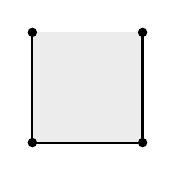
\begin{tikzpicture}[
    x=0.7cm,y=0.7cm,
    font=\small,
    line cap=round,
    line join=round,
    vertex/.style={circle,fill,inner sep=1.2pt},
    ambient/.style={draw=gray!55, line width=0.45pt},
    mainedge/.style={draw=black, line width=0.8pt}
]

\coordinate (A) at (0,0);
\coordinate (B) at (2.0,0);
\coordinate (C) at (0,2.0);
\coordinate (D) at (2.0,2.0);

\fill[gray!15] (A)--(B)--(D)--(C)--cycle;

\draw[mainedge] (A)--(B);
\draw[mainedge] (A)--(C);
\draw[mainedge] (B)--(D);

\foreach \P in {A,B,C,D} {
    \node[vertex] at (\P) {};
}

\end{tikzpicture}
	\end{center}
	and is clearly not a trivial cofibration.
\end{example}

\begin{remark}
	Note that this U-shape is precisely the horn in classical cubical homotopy theory,
	see~\cite[Definition 10.3.2]{Brown2011}.
\end{remark}

This shows that the pushout product of a trivial cofibration with a general (normal) monomorphism is not necessarily a trivial cofibration.



\subsubsection{Cubesets with Gluing Property}

Given two $n$-cubes, we can glue them along an ($n-1$)-dimensional face (an inert $\epsilon_i\colon{\bbox}^{n-1}\to{\bbox}^n$) to obtain ${\bbox}^n\sqcup_{{\bbox}^{n-1}}{\bbox}^n$.
Opposite to where we have glued, we obtain a map ${\bbox}^{n-1}\sqcup{\bbox}^{n-1}\to{\bbox}^n\sqcup_{{\bbox}^{n-1}}{\bbox}^n$ induced by the \emph{upper face map} $\overline{\epsilon}_i\colon{\bbox}^{n-1}\to{\bbox}^n$
which is $\epsilon_i$ but with the $0$ swapped for a $1$.
This map can be glued along the map $\epsilon_i\sqcup\overline{\epsilon}_i\colon{\bbox}^{n-1}\sqcup{\bbox}^{n-1}\to{\bbox}^n$,
so that we obtain a pushout square
\begin{center}
\begin{tikzcd}
	{{\bbox}^{n-1}\sqcup{\bbox}^{n-1}} & {{\bbox}^n} \\
	{{\bbox}^{n}\sqcup_{{\bbox}^{n-1}}{\bbox}^{n}} & {({\bbox}^{n}\sqcup_{{\bbox}^{n-1}}{\bbox}^{n})\sqcup_{{\bbox}^{n-1}\sqcup{\bbox}^{n-1}}{\bbox}^n}
	\arrow[from=1-1, to=1-2]
	\arrow[from=1-1, to=2-1]
	\arrow[from=1-2, to=2-2]
	\arrow[from=2-1, to=2-2]
\end{tikzcd}
\end{center}
where the lower horizontal map is a monomorphism since the upper one is.
This allows us to define the set of morphisms
\[
    \bprism\coloneq \{ {{\bbox}^{n}\sqcup_{{\bbox}^{n-1}}{\bbox}^{n}}\to{({\bbox}^{n}\sqcup_{{\bbox}^{n-1}}{\bbox}^{n})\sqcup_{{\bbox}^{n-1}\sqcup{\bbox}^{n-1}}{\bbox}^n} \mid n\in\N \}.
\]

\begin{definition}\label{def:gluing-property}
A cubeset $X$ has the \emph{gluing property} if the map $p\colon X\to\ast$ has the right lifting property w.r.t. $\bprism$.
Moreover we say that $X$ has \emph{unique gluing} if the lift is unique (and exists, i.e. the object is local with respect to $\bprism$).
	We say that $X$ has \emph{at most unique gluing} if the lift is unique whenever it exists.
\end{definition}

\begin{proposition}\label{prop:unique-gluing-concrete}
A cubeset $X$ has at most unique gluing if and only if it is concrete.
\end{proposition}

\begin{proof}
The if direction is clear.
For the only if direction we argue by induction on the dimension $n$.
For $n=1$, we need to show that for two points $a,b\in X(0)$
there is at most one edge with these two boundary points.
Consider some edge $f$ between $a$ and $b$, and glue it to the degenerate $a$-cube.
Therefore, $f$ is a gluing of $f$ and the degenerate cube.
Now, any other $g$ between $a$ and $b$ also is a gluing of $f$ and the degenerate $a$-cube,
so we have $f=g$
\begin{center}
\begin{tikzcd}[row sep=tiny,column sep=tiny]
	a && \\
	\\
	a && b
	\arrow["e", no head, from=3-1, to=1-1]
	\arrow["f"', no head, from=3-1, to=3-3]
	\arrow["f"', shift right, no head, from=3-3, to=1-1]
	\arrow["g", shift left, no head, from=3-3, to=1-1]
\end{tikzcd}.
\end{center}
Thus, the map $X(1)\to X(0)^2$ is injective.
For a general dimension we argue similarly: Consider two $n$-cubes $f$ and $g$ with the same points.
Then by induction, all their faces of dimension $n-1$ agree.
Now, take any face of $f$ and consider the degenerate $n$-cube of this face.
Then, $f$ and $g$ both yield gluings of this degenerate cube and of $f$, and thus $g=f$.
\begin{center}
\begin{tikzcd}[ampersand replacement=\&,sep=small]
	\& \bullet \&\&\& \\
	\bullet \\
	\\
	\& \bullet \&\&\& \bullet \\
	\bullet \&\&\& \bullet
	\arrow[""{name=0, anchor=center, inner sep=0}, no head, from=1-2, to=4-5]
	\arrow[""{name=1, anchor=center, inner sep=0}, curve={height=-12pt}, no head, from=1-2, to=4-5]
	\arrow["a"{description}, no head, from=2-1, to=1-2]
	\arrow[""{name=2, anchor=center, inner sep=0}, no head, from=2-1, to=5-4]
	\arrow[""{name=3, anchor=center, inner sep=0}, curve={height=-12pt}, no head, from=2-1, to=5-4]
	\arrow[no head, from=4-2, to=1-2]
	\arrow[""{name=4, anchor=center, inner sep=0}, no head, from=4-2, to=4-5]
	\arrow[no head, from=5-1, to=2-1]
	\arrow["a"{description}, no head, from=5-1, to=4-2]
	\arrow[""{name=5, anchor=center, inner sep=0}, no head, from=5-1, to=5-4]
	\arrow[no head, from=5-4, to=4-5]
	\arrow["f"{description}, shift right=2, draw=none, from=2, to=0]
	\arrow["g"{description}, shift left=2, draw=none, from=3, to=1]
	\arrow["f"', shift left=4, draw=none, from=5, to=4]
\end{tikzcd}
\end{center}
\end{proof}

\begin{proposition}\label{prop:nilfib-gluing}
Let $X$ be a fibrant cubeset. Then $X$ has the gluing property.
\end{proposition}

\begin{proof}
We simply embed the 2-roof $\bbcor^2\times \bbox^{n-1}\to \bbox^2\times \bbox^{n-1}$ and then restrict to the triangle which includes the off-diagonal of the $2$-square.
This is the same as the inclusion used in the gluing property.

\pgfdeclarelayer{facefill}
\pgfdeclarelayer{faceoutline}
\pgfsetlayers{facefill,faceoutline,main}
\begin{center}
\newcommand{\DarkFace}[1]{%
  \begin{pgfonlayer}{facefill}
    \path[fill=gray, fill opacity=0.24] #1 -- cycle;
  \end{pgfonlayer}
  \begin{pgfonlayer}{faceoutline}
    \path[draw=gray!70,line width=0.5pt] #1 -- cycle;
  \end{pgfonlayer}
}

\newcommand{\PrismFace}[1]{%
  \begin{pgfonlayer}{facefill}
    \path[fill=blue!20!gray, fill opacity=0.24] #1 -- cycle;
  \end{pgfonlayer}
  \begin{pgfonlayer}{faceoutline}
    \path[draw=blue!35!black,line width=0.5pt] #1 -- cycle;
  \end{pgfonlayer}
}

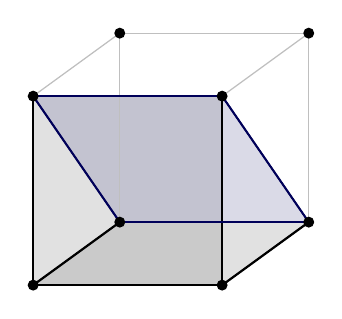
\begin{tikzpicture}[
    x=1cm,y=1cm,
    font=\small,
    line cap=round,
    line join=round,
    vertex/.style={circle,fill,inner sep=1.4pt},
    ambient/.style={draw=gray!50, line width=0.45pt},
    mainedge/.style={draw=black, line width=0.8pt},
    prismedge/.style={draw=blue!35!black, line width=0.75pt}
]

\coordinate (A) at (0,0);
\coordinate (B) at (2.4,0);
\coordinate (C) at (0,2.4);
\coordinate (D) at (2.4,2.4);

\coordinate (E) at (1.1,0.8);
\coordinate (F) at (3.5,0.8);
\coordinate (G) at (1.1,3.2);
\coordinate (H) at (3.5,3.2);


\draw[ambient] (A)--(B)--(D)--(C)--cycle;
\draw[ambient] (E)--(F)--(H)--(G)--cycle;
\draw[ambient] (A)--(E);
\draw[ambient] (B)--(F);
\draw[ambient] (C)--(G);
\draw[ambient] (D)--(H);


\DarkFace{(A)--(B)--(D)--(C)}
\DarkFace{(A)--(B)--(F)--(E)}

\PrismFace{(C)--(D)--(F)--(E)}

\draw[mainedge] (A)--(B);
\draw[mainedge] (B)--(D);
\draw[mainedge] (D)--(C);
\draw[mainedge] (C)--(A);

\draw[mainedge] (A)--(B);
\draw[mainedge] (B)--(F);
\draw[mainedge] (F)--(E);
\draw[mainedge] (E)--(A);

\draw[prismedge] (C)--(D);
\draw[prismedge] (D)--(F);
\draw[prismedge] (F)--(E);
\draw[prismedge] (E)--(C);

\foreach \P in {A,B,C,D,E,F,G,H} {
    \node[vertex] at (\P) {};
}

\end{tikzpicture}
\end{center}
Hence, a gluing may be computed from fibrancy by taking the off-diagonals of a lift of the roof
$\bbox^{n-1}\times \bbcor^2\hookrightarrow \bbox^{n+1}$.
\end{proof}

\begin{corollary}
Concrete fibrant cubesets are precisely the fibrant cubesets with unique gluing property.
\end{corollary}

\begin{lemma}
The subcategory of cubespaces with unique gluing property forms a reflective subcategory of all cubesets, i.e. the inclusion admits a left adjoint.
\end{lemma}

\begin{proof}
This follows from the fact that cubesets with unique gluing property are the $\bprism$-local objects,
and on local objects there is always a reflection, see \cite[Theorem 1.39]{Adamek1994}.
\end{proof}



\subsubsection{Fibrations over \texorpdfstring{$\bbGamma$}{Gamma}}\label{ssec:corner-gamma}

In this section we work in the opposite category $\bbGamma$ of finite pointed sets, unless otherwise noted.
Recall that it can be interpreted as a wide subcategory $\bblox$ of the whole cube category $\bbox$
where the morphisms fix the base point.
In this category, there is another definition of $n$-corner than in the whole $\bbox$.
Recall that we denote by ${\bblox}^n$ the image of $\langle n\rangle$ under the Yoneda embedding
$\bbGamma\to\PSh(\bbGamma)$ and by ${\bbox}^n$ the image of $\{0,1\}^n$ under the Yoneda embedding
$\bbox\to\cSet$.

\begin{definition}\label{def:omega_corner_gamma}
Let $n\in\N$ and $\omega\in\{0,1\}^n\setminus\{0^n\}$.
Then define the $n$-corner ${\bbcor}^n_\omega$ w.r.t. $\omega$ as the union over all injections $f\colon{\bblox}^{n-1}\to{\bblox}^n$ in $\bbGamma$
such that $f$ misses $\omega$, i.e., $\omega\notin\im f$:
\[
    {\bbcor}^n_\omega = \bigcup_{\substack{f\colon{\bblox}^{n-1}\sub{\bblox}^n \\ \omega\notin\im f}}{\bblox}^{n-1}\hookrightarrow{\bblox}^n.
\]
\end{definition}

\begin{example}
In two dimensions, the corners look like
\begin{center}
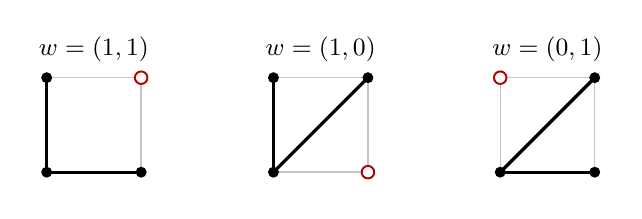
\begin{tikzpicture}[
    scale=0.6,
    line cap=round,
    line join=round,
    bg/.style={draw=gray!45, line width=0.5pt},
    face/.style={draw=black, line width=1.2pt},
    vtx/.style={circle, fill=black, inner sep=1.4pt},
    missing/.style={circle, draw=red!70!black, fill=white, line width=0.7pt, inner sep=1.6pt},
    lab/.style={font=\scriptsize},
    title/.style={font=\small\bfseries}
]
\begin{scope}[shift={(0,0)}]
  \node[title] at (1,2.6) {$w=(1,1)$};

  \coordinate (O) at (0,0);
  \coordinate (A) at (2,0);
  \coordinate (B) at (0,2);
  \coordinate (C) at (2,2);

  \draw[bg] (O)--(A)--(C)--(B)--cycle;

  \draw[face] (O)--(A);
  \draw[face] (O)--(B);

  \node[vtx] at (O) {};
  \node[vtx] at (A) {};
  \node[vtx] at (B) {};
  \node[missing] at (C) {};

  \node[lab, below left]  at (O) {};
  \node[lab, below right] at (A) {};
  \node[lab, above left]  at (B) {};
  \node[lab, above right] at (C) {};
\end{scope}

\begin{scope}[shift={(4.8,0)}]
  \node[title] at (1,2.6) {$w=(1,0)$};

  \coordinate (O) at (0,0);
  \coordinate (A) at (2,0);
  \coordinate (B) at (0,2);
  \coordinate (C) at (2,2);

  \draw[bg] (O)--(A)--(C)--(B)--cycle;

  \draw[face] (O)--(B);
  \draw[face] (O)--(C);

  \node[vtx] at (O) {};
  \node[missing] at (A) {};
  \node[vtx] at (B) {};
  \node[vtx] at (C) {};

  \node[lab, below left]  at (O) {};
  \node[lab, below right] at (A) {};
  \node[lab, above left]  at (B) {};
  \node[lab, above right] at (C) {};
\end{scope}


\begin{scope}[shift={(9.6,0)}]
  \node[title] at (1,2.6) {$w=(0,1)$};

  \coordinate (O) at (0,0);
  \coordinate (A) at (2,0);
  \coordinate (B) at (0,2);
  \coordinate (C) at (2,2);

  \draw[bg] (O)--(A)--(C)--(B)--cycle;

  \draw[face] (O)--(A);
  \draw[face] (O)--(C);

  \node[vtx] at (O) {};
  \node[vtx] at (A) {};
  \node[missing] at (B) {};
  \node[vtx] at (C) {};

  \node[lab, below left]  at (O) {};
  \node[lab, below right] at (A) {};
  \node[lab, above left]  at (B) {};
  \node[lab, above right] at (C) {};
\end{scope}

\end{tikzpicture}
\end{center}
And the three-dimensional case looks as follows.
\begin{center}
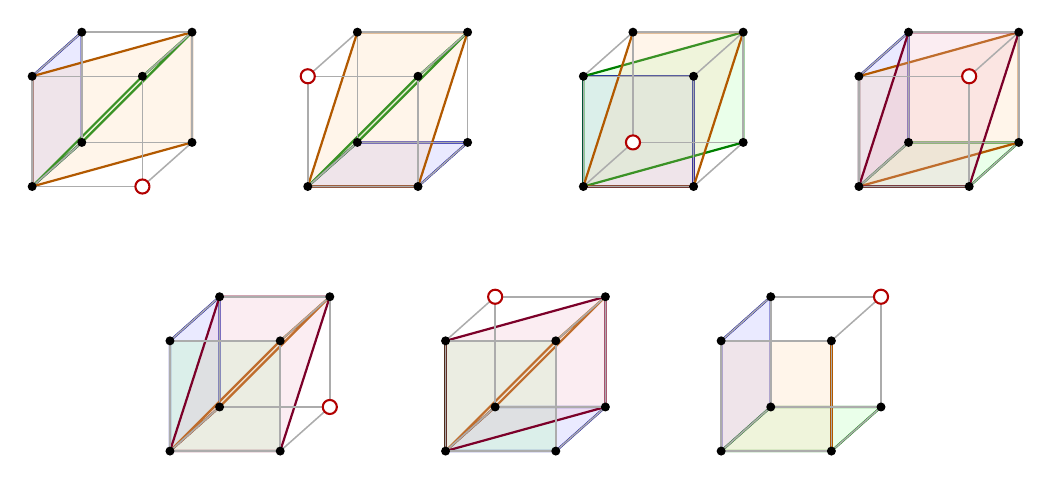
\begin{tikzpicture}[
    scale=0.7,
    line cap=round,
    line join=round,
    edge/.style={draw=gray!65, line width=0.55pt},
    frontedge/.style={draw=black, line width=0.65pt},
    vertex/.style={circle, fill=black, inner sep=1.15pt},
    missing/.style={circle, draw=red!70!black, fill=white, line width=0.75pt, inner sep=1.8pt},
    faceA/.style={fill=blue!35,   draw=blue!60!black,   fill opacity=0.23, line width=0.8pt},
    faceB/.style={fill=green!35,  draw=green!50!black,  fill opacity=0.23, line width=0.8pt},
    faceC/.style={fill=orange!35, draw=orange!70!black, fill opacity=0.23, line width=0.8pt},
    faceD/.style={fill=purple!30, draw=purple!65!black, fill opacity=0.23, line width=0.8pt}
]


\begin{scope}[shift={(0,4.8)}]
  \coordinate (A) at (0,0);
  \coordinate (B) at (2,0);
  \coordinate (C) at (0,2);
  \coordinate (D) at (2,2);
  \coordinate (E) at (0.9,0.8);
  \coordinate (F) at (2.9,0.8);
  \coordinate (G) at (0.9,2.8);
  \coordinate (H) at (2.9,2.8);

  \filldraw[faceA] (A)--(C)--(G)--(E)--cycle;
  \filldraw[faceB] (A)--(D)--(H)--(E)--cycle;
  \filldraw[faceC] (A)--(C)--(H)--(F)--cycle;

  \draw[edge] (A)--(B)--(D)--(C)--cycle;
  \draw[edge] (E)--(F)--(H)--(G)--cycle;
  \draw[edge] (A)--(E);
  \draw[edge] (B)--(F);
  \draw[edge] (C)--(G);
  \draw[edge] (D)--(H);

  \node[vertex]  at (A) {};
  \node[missing] at (B) {};
  \node[vertex]  at (C) {};
  \node[vertex]  at (D) {};
  \node[vertex]  at (E) {};
  \node[vertex]  at (F) {};
  \node[vertex]  at (G) {};
  \node[vertex]  at (H) {};
\end{scope}


\begin{scope}[shift={(5.0,4.8)}]
  \coordinate (A) at (0,0);
  \coordinate (B) at (2,0);
  \coordinate (C) at (0,2);
  \coordinate (D) at (2,2);
  \coordinate (E) at (0.9,0.8);
  \coordinate (F) at (2.9,0.8);
  \coordinate (G) at (0.9,2.8);
  \coordinate (H) at (2.9,2.8);

  \filldraw[faceA] (A)--(B)--(F)--(E)--cycle;
  \filldraw[faceB] (A)--(D)--(H)--(E)--cycle;
  \filldraw[faceC] (A)--(B)--(H)--(G)--cycle;

  \draw[edge] (A)--(B)--(D)--(C)--cycle;
  \draw[edge] (E)--(F)--(H)--(G)--cycle;
  \draw[edge] (A)--(E);
  \draw[edge] (B)--(F);
  \draw[edge] (C)--(G);
  \draw[edge] (D)--(H);

  \node[vertex]  at (A) {};
  \node[vertex]  at (B) {};
  \node[missing] at (C) {};
  \node[vertex]  at (D) {};
  \node[vertex]  at (E) {};
  \node[vertex]  at (F) {};
  \node[vertex]  at (G) {};
  \node[vertex]  at (H) {};
\end{scope}


\begin{scope}[shift={(10.0,4.8)}]
  \coordinate (A) at (0,0);
  \coordinate (B) at (2,0);
  \coordinate (C) at (0,2);
  \coordinate (D) at (2,2);
  \coordinate (E) at (0.9,0.8);
  \coordinate (F) at (2.9,0.8);
  \coordinate (G) at (0.9,2.8);
  \coordinate (H) at (2.9,2.8);

  \filldraw[faceA] (A)--(B)--(D)--(C)--cycle;
  \filldraw[faceB] (A)--(C)--(H)--(F)--cycle;
  \filldraw[faceC] (A)--(B)--(H)--(G)--cycle;

  \draw[edge] (A)--(B)--(D)--(C)--cycle;
  \draw[edge] (E)--(F)--(H)--(G)--cycle;
  \draw[edge] (A)--(E);
  \draw[edge] (B)--(F);
  \draw[edge] (C)--(G);
  \draw[edge] (D)--(H);

  \node[vertex]  at (A) {};
  \node[vertex]  at (B) {};
  \node[vertex]  at (C) {};
  \node[vertex]  at (D) {};
  \node[missing] at (E) {};
  \node[vertex]  at (F) {};
  \node[vertex]  at (G) {};
  \node[vertex]  at (H) {};
\end{scope}


\begin{scope}[shift={(15.0,4.8)}]
  \coordinate (A) at (0,0);
  \coordinate (B) at (2,0);
  \coordinate (C) at (0,2);
  \coordinate (D) at (2,2);
  \coordinate (E) at (0.9,0.8);
  \coordinate (F) at (2.9,0.8);
  \coordinate (G) at (0.9,2.8);
  \coordinate (H) at (2.9,2.8);

  \filldraw[faceA] (A)--(C)--(G)--(E)--cycle;
  \filldraw[faceB] (A)--(B)--(F)--(E)--cycle;
  \filldraw[faceC] (A)--(C)--(H)--(F)--cycle;
  \filldraw[faceD] (A)--(B)--(H)--(G)--cycle;

  \draw[edge] (A)--(B)--(D)--(C)--cycle;
  \draw[edge] (E)--(F)--(H)--(G)--cycle;
  \draw[edge] (A)--(E);
  \draw[edge] (B)--(F);
  \draw[edge] (C)--(G);
  \draw[edge] (D)--(H);

  \node[vertex]  at (A) {};
  \node[vertex]  at (B) {};
  \node[vertex]  at (C) {};
  \node[missing] at (D) {};
  \node[vertex]  at (E) {};
  \node[vertex]  at (F) {};
  \node[vertex]  at (G) {};
  \node[vertex]  at (H) {};
\end{scope}


\begin{scope}[shift={(2.5,0)}]
  \coordinate (A) at (0,0);
  \coordinate (B) at (2,0);
  \coordinate (C) at (0,2);
  \coordinate (D) at (2,2);
  \coordinate (E) at (0.9,0.8);
  \coordinate (F) at (2.9,0.8);
  \coordinate (G) at (0.9,2.8);
  \coordinate (H) at (2.9,2.8);

  \filldraw[faceA] (A)--(C)--(G)--(E)--cycle;
  \filldraw[faceB] (A)--(B)--(D)--(C)--cycle;
  \filldraw[faceC] (A)--(D)--(H)--(E)--cycle;
  \filldraw[faceD] (A)--(B)--(H)--(G)--cycle;

  \draw[edge] (A)--(B)--(D)--(C)--cycle;
  \draw[edge] (E)--(F)--(H)--(G)--cycle;
  \draw[edge] (A)--(E);
  \draw[edge] (B)--(F);
  \draw[edge] (C)--(G);
  \draw[edge] (D)--(H);

  \node[vertex]  at (A) {};
  \node[vertex]  at (B) {};
  \node[vertex]  at (C) {};
  \node[vertex]  at (D) {};
  \node[vertex]  at (E) {};
  \node[missing] at (F) {};
  \node[vertex]  at (G) {};
  \node[vertex]  at (H) {};
\end{scope}


\begin{scope}[shift={(7.5,0)}]
  \coordinate (A) at (0,0);
  \coordinate (B) at (2,0);
  \coordinate (C) at (0,2);
  \coordinate (D) at (2,2);
  \coordinate (E) at (0.9,0.8);
  \coordinate (F) at (2.9,0.8);
  \coordinate (G) at (0.9,2.8);
  \coordinate (H) at (2.9,2.8);

  \filldraw[faceA] (A)--(B)--(F)--(E)--cycle;
  \filldraw[faceB] (A)--(B)--(D)--(C)--cycle;
  \filldraw[faceC] (A)--(D)--(H)--(E)--cycle;
  \filldraw[faceD] (A)--(C)--(H)--(F)--cycle;

  \draw[edge] (A)--(B)--(D)--(C)--cycle;
  \draw[edge] (E)--(F)--(H)--(G)--cycle;
  \draw[edge] (A)--(E);
  \draw[edge] (B)--(F);
  \draw[edge] (C)--(G);
  \draw[edge] (D)--(H);

  \node[vertex]  at (A) {};
  \node[vertex]  at (B) {};
  \node[vertex]  at (C) {};
  \node[vertex]  at (D) {};
  \node[vertex]  at (E) {};
  \node[vertex]  at (F) {};
  \node[missing] at (G) {};
  \node[vertex]  at (H) {};
\end{scope}


\begin{scope}[shift={(12.5,0)}]
  \coordinate (A) at (0,0);
  \coordinate (B) at (2,0);
  \coordinate (C) at (0,2);
  \coordinate (D) at (2,2);
  \coordinate (E) at (0.9,0.8);
  \coordinate (F) at (2.9,0.8);
  \coordinate (G) at (0.9,2.8);
  \coordinate (H) at (2.9,2.8);

  \filldraw[faceA] (A)--(C)--(G)--(E)--cycle;
  \filldraw[faceB] (A)--(B)--(F)--(E)--cycle;
  \filldraw[faceC] (A)--(B)--(D)--(C)--cycle;

  \draw[edge] (A)--(B)--(D)--(C)--cycle;
  \draw[edge] (E)--(F)--(H)--(G)--cycle;
  \draw[edge] (A)--(E);
  \draw[edge] (B)--(F);
  \draw[edge] (C)--(G);
  \draw[edge] (D)--(H);

  \node[vertex]  at (A) {};
  \node[vertex]  at (B) {};
  \node[vertex]  at (C) {};
  \node[vertex]  at (D) {};
  \node[vertex]  at (E) {};
  \node[vertex]  at (F) {};
  \node[vertex]  at (G) {};
  \node[missing] at (H) {};
\end{scope}
\end{tikzpicture}
\end{center}
\end{example}

For every dimension $n$ there are thus $2^n-1$ corners.
However, as the next proposition shows, there essentially are only $n$ relevant corners.
Let $d_\omega = \lvert\omega\rvert$ be the distance of $\omega$ to $0^n$.

\begin{proposition}
Let $n\in\N$ and $\omega,\epsilon\in\{0,1\}^n\setminus\{0^n\}$.
Then there is an automorphism $\phi$ on ${\bblox}^n$ in $\bbGamma$ such that the induced function $\mathrm{Sub}({\bblox}^n)\to\mathrm{Sub}({\bblox}^n)$
maps ${\bbcor}^n_\omega$ to ${\bbcor}^n_\epsilon$ precisely if $d_\omega = d_\epsilon$.
\end{proposition}

\begin{proof}
If $d_\omega = d_\epsilon$, there exists an automorphism $\phi$ of ${\bblox}^n$ in $\bbGamma$ with $\phi(\omega) = \epsilon$,
given by permuting the corresponding coordinates (since there are equally many 1's in $\omega$ as in $\epsilon$).
Now we need to see that the composition ${\bbcor}^n_\omega\to{\bblox}^n\to{\bblox}^n$ corresponds to ${\bbcor}^n_\epsilon\sub{\bblox}^n$.
Since $\phi$ is an isomorphism, it induces a bijection of subobjects.
Thus, for $f\colon{\bblox}^{n-1}\hookrightarrow{\bblox}^n$, $\omega\notin\im f$ precisely if $\epsilon\notin\im g$ for $g = \phi\circ f$.
Therefore, the unions are the same and so $\phi$ maps ${\bbcor}^n_\omega$ to ${\bbcor}^n_\epsilon$.
\end{proof}

\begin{definition}\label{def:corner_in_gamma}
We define
\[
    \Lambda_{\bbGamma} \coloneq \{{\bbcor}^n_\omega\hookrightarrow{\bblox}^n \mid n\in\N,\,\omega\in\{0,1\}^n\setminus\{0^n\}\}.
\]
\end{definition}

A priori, given a cubeset $X$, its underlying $\bbGamma$-set $j^\ast X$ (see Remark~\ref{rem:adjoint-triple-j})
supports a different notion of fibrancy w.r.t. $\Lambda_{\bbGamma}$.
However, in the concrete setting, there is no difference as the next proposition shows.

\begin{proposition}\label{prop:nilfib-restricted-nilfib-concrete}
Let $X$ be a concrete cubeset.
Then the following assertions are equivalent.
\begin{enumerate}[(a)]
    \item The cubeset $X$ is fibrant.
    \item The projection $p\colon j^\ast X\to\ast$ has the right lifting property against
        $\Lambda_{\bbGamma}$, i.e. the underlying $\bbGamma$-set is fibrant w.r.t. $\Lambda_{\bbGamma}$.
\end{enumerate}
\end{proposition}

\begin{proof}
By adjunction, a diagonal lift in the left diagram (in $\PSh(\bbGamma)$) corresponds to a lift in the right diagram (in $\cSet$):
\begin{center}
\begin{tikzcd}
	{{\bbcor}^n_\omega} & {j^\ast X} & {j_!{\bbcor}^n_\omega} & X \\
	{{\bblox}^n} & \ast & {j_!{\bblox}^n} & \ast
	\arrow[from=1-1, to=1-2]
	\arrow[from=1-1, to=2-1]
	\arrow[""{name=0, anchor=center, inner sep=0}, from=1-2, to=2-2]
	\arrow[from=1-3, to=1-4]
	\arrow[""{name=1, anchor=center, inner sep=0}, from=1-3, to=2-3]
	\arrow[from=1-4, to=2-4]
	\arrow[dashed, from=2-1, to=1-2]
	\arrow[from=2-1, to=2-2]
	\arrow[dashed, from=2-3, to=1-4]
	\arrow[from=2-3, to=2-4]
	\arrow["\leftrightsquigarrow"{description}, draw=none, from=0, to=1]
\end{tikzcd}
\end{center}
But $j_!{\bblox}^n = {\bbox}^n$ and by Lemma~\ref{lem:j-geometric-morphism}, $j_!$ preserves finite unions of subobjects
(the union of subobjects is the pushout of those subobjects along their intersection), so we have that
\[
    j_!{\bbcor}^n_\omega = \bigcup_{\substack{f\colon{\bbox}^{n-1}\sub{\bbox}^n \\ f\in\PSh(\bbGamma) \\ \omega\notin\im f}}{\bbox}^{n-1}
\]
where the union now is taken in $\cSet$ instead of $\PSh(\bbGamma)$.
Note that for $\omega=1^n$ this just corresponds to the classical corner ${\bbcor}^n$ in $\cSet$:
If $f\colon{\bbox}^{n-1}\hookrightarrow{\bbox}^n$ is a linear (= base point preserving) injective map in $\bbox$ with $1^n\notin\im f$,
then by its canonical representation we know that each $x_i$ appears at least once, and there must be at least one constant $0$.
In particular, by dimension, every $x_i$ appears exactly once, so $f=\epsilon_k$ for some $k$.
Here, $\epsilon_k$ is the inert map corresponding to the $k$-th coordinate.
Thus, $j_!{\bbcor}^n_{1^n} = {\bbcor}^n$.
This directly yields the implication $(b)\implies (a)$.

The other direction requires a bit more work for which we first develop the setup.
\end{proof}

We now want to mimic the definition of $\Lambda_{\bbGamma}$ in $\PSh(\bbGamma)$ also in $\cSet$.

\begin{definition}
Let $n\in\N$ and $\omega\in\{0,1\}^n\setminus\{0^n\}$.
Then define the $n$-corner ${\bbcor}^n_\omega$ w.r.t. $\omega$ as the union over all injections
$f\colon{\bbox}^{n-1}\to{\bbox}^n$ in $\bbox$ such that $f$ misses $\omega$, i.e., $\omega\notin\im f$:
\[
    {\bbcor}^n_\omega = \bigcup_{\substack{f\colon{\bbox}^{n-1}\sub{\bbox}^n \\ \omega\notin\im f}}{\bbox}^{n-1}\hookrightarrow{\bbox}^n.
\]
We define
\[
    \Lambda' \coloneq \{{\bbcor}^n_\omega\hookrightarrow{\bbox}^n \mid n\in\N,\,\omega\in\{0,1\}^n\setminus\{0^n\}\}
\]
as a set of morphisms in $\cSet$.
\end{definition}

\begin{lemma}\label{lem:alternative-nilfibrant-concrete}
Let $X$ be a concrete cubeset with the gluing property and consider the projection $p\colon X\to\ast$.
Then the following assertions are equivalent.
\begin{enumerate}[(a)]
    \item $p$ has the right lifting property w.r.t. $\Lambda'$.
    \item $p$ has the right lifting property w.r.t. $\Lambda$, i.e., $X$ is fibrant.
\end{enumerate}
\end{lemma}

\begin{proof}
$(a)\implies(b)$:
Let $\lambda\colon{\bbcor}^n\to X$ be an $n$-corner in $X$.
For every subobject $f\colon{\bbox}^{n-1}\to{\bbox}^n$ that misses $1^n$ and is not an inert,
there exists an $i$ such that $x_i$ appears twice in the canonical representation of $f$,
once as $x_i$ (at coordinate $k$) and once as $1-x_i$ (at coordinate $j$).
Then $f\lvert_{[x_i=0]}$ factors through the inert $\epsilon_k$ as an $n-2$-dimensional cube,
and $f\lvert_{[x_i=1]}$ factors through the inert $\epsilon_j$ as an $n-2$-dimensional cube.
Restricting the corner to $\epsilon_k\cup\epsilon_j$ yields a map ${\bbox}^{n-1}\sqcup_{{\bbox}^{n-2}}{\bbox}^{n-1}\to X$.
Since $X$ has the (unique) gluing property, we can extend it (uniquely) to a map
\[
    ({\bbox}^{n-1}\sqcup_{{\bbox}^{n-2}}{\bbox}^{n-1})\sqcup_{{\bbox}^{n-2}\sqcup{\bbox}^{n-2}}{\bbox}^{n-1}\to X
\]
whose restriction to ${\bbox}^{n-1}$ can be viewed as an extension of $\lambda$ to (the image of) $f$.
Iterating this process exhausts, after finitely many steps, all injective non-inert maps ${\bbox}^{n-1}\to{\bbox}^n$ that miss $1^n$,
compatible on intersections (by the uniqueness of the gluings),
and thus gives a map $\lambda'\colon{\bbcor}^n_{1^n}\to X$ that restricts to $X$.
This map $\lambda'$ can, by assumption, be lifted to a cube in $X$ which then also is a completion of $\lambda$.

$(b)\implies(a)$:
By applying an automorphism, we may assume that $\omega = 1^n$.
So we need to see that $p$ lifts against ${\bbcor}^n_{1^n}\to{\bbox}^n$.
Restricting to ${\bbcor}^n$ yields a lift
\begin{center}
\begin{tikzcd}
	{{\bbcor}^n} & X \\
	{{\bbcor}^n_{1^n}} & X \\
	{{\bbox}^n} & \ast
	\arrow[from=1-1, to=1-2]
	\arrow[from=1-1, to=2-1]
	\arrow[from=2-1, to=2-2]
	\arrow[from=2-1, to=3-1]
	\arrow["\id"', from=2-2, to=1-2]
	\arrow[from=2-2, to=3-2]
	\arrow[dashed, from=3-1, to=1-2]
	\arrow[from=3-1, to=3-2]
\end{tikzcd}
\end{center}
making the outer rectangle and triangles commutative.
Since $X$ is concrete, also the lower small triangle commutes:
the values of the corner completion on an antidiagonal in ${\bbcor}^n_{1^n}$ not in ${\bbcor}^n$
are uniquely determined by its values on points, which already are present in ${\bbcor}^n$.
\end{proof}

\begin{lemma}\label{lem:different-liftings-comparison}
We have the following inclusion
\[
    j_!(\Lambda_{\bbGamma})\subset\mathrm{sat}(\Lambda'\cup\bprism)
\]
of morphisms in $\cSet$.
\end{lemma}

\begin{proof}
Let $f\in\Lambda_{\bbGamma}$ be a map $f\colon{\bbcor}^n_\omega\to{\bblox}^n$.
We first extend $j_!f$ along outer faces that don't contain $\omega$,
using pushouts along maps in $\bprism$,
such that, after applying an automorphism of the cube mapping $\omega$ to $1^n$,
the domain of the extended $j_!f$ contains the classical corner ${\bbcor}^n$.
Lastly, we extend $j_!f$ to all anti-diagonals, using pushouts along maps in $\bprism$.
This procedure thus has extended $j_!f$ to a map in $\Lambda'$, yielding the claim.

Assume that there is an inert $\epsilon_i\colon{\bbox}^{n-1}\to{\bbox}^n$ such that $\omega_i = 0$,
i.e., $\omega\in\epsilon_i$.
Now take some $k$ with $\omega_k = 1$.
Then $\epsilon_k$ factors through ${\bbcor}^n_\omega$.
Define $s_k\colon{\bbox}^{n-1}\to{\bbox}^n$ by
\[
    s_k(x_1,\ldots,x_{n-1})\mapsto (x_1,\ldots,x_k,x_{k+1},\dots,x_{i-1}, x_k, x_{i}\ldots,x_{n-1})
\]
where the second $x_k$ appears at index $i$, having image $[x_k=x_i]$ (for $i<k$ swap them).
Since $s_k$ is linear and doesn't contain $\omega$, it factors through ${\bbcor}^n_\omega$.
Moreover, $\epsilon_k\cap s_k$ is isomorphic to ${\bbox}^{n-2}$,
so we obtain a map $(\epsilon_k,s_k)\colon{\bbox}^{n-1}\sqcup_{{\bbox}^{n-2}}{\bbox}^{n-1}\to{\bbcor}^n_\omega$.
Now $\epsilon_k\cap\overline{\epsilon}_i$ and $s_k\cap\overline{\epsilon}_i$ both are isomorphic to ${\bbox}^{n-2}$,
and their intersection as subobjects of ${\bbox}^n$ is empty.
This induces a map $({\bbox}^{n-1}\sqcup_{{\bbox}^{n-2}}{\bbox}^{n-1})\sqcup_{{\bbox}^{n-2}\sqcup{\bbox}^{n-2}}{\bbox}^{n-1}\to{\bbox}^n$
which on the left acts as $(\epsilon_k,s_k)$ and on the right as $\overline{\epsilon}_i$.
This map makes the outer square commutative
\begin{center}
\begin{tikzcd}
	{{\bbox}^{n-1}\sqcup_{{\bbox}^{n-2}}{\bbox}^{n-1}} && {{\bbcor}^n_\omega} & \\
	\\
	{({\bbox}^{n-1}\sqcup_{{\bbox}^{n-2}}{\bbox}^{n-1})\sqcup_{{\bbox}^{n-2}\sqcup{\bbox}^{n-2}}{\bbox}^{n-1}} && {X_i} \\
	&&& {{\bbox}^n}
	\arrow[""{name=0, anchor=center, inner sep=0}, from=1-1, to=1-3]
	\arrow[from=1-1, to=3-1]
	\arrow[from=1-3, to=3-3]
	\arrow["j_!f", from=1-3, to=4-4]
	\arrow[from=3-1, to=3-3]
	\arrow[from=3-1, to=4-4]
	\arrow[dashed, from=3-3, to=4-4]
	\arrow["\lrcorner"{anchor=center, pos=0.125, rotate=180}, draw=none, from=3-3, to=0]
\end{tikzcd}.
\end{center}
Taking the pushout $X_i$ gives a factorization of $j_!f$ where the first map
is in $\mathrm{sat}(\Lambda'\cup\bprism)$ (since the left vertical map is in $\bprism$),
and all maps are injective.
Now repeat this process for all $i$ with $\omega_i=0$.
This yields a factorization
\begin{center}
\begin{tikzcd}
	{{\bbcor}^n_\omega} & X & {{\bbox}^n}
	\arrow["h"', from=1-1, to=1-2]
	\arrow["j_!f", curve={height=-12pt}, from=1-1, to=1-3]
	\arrow["g"', from=1-2, to=1-3]
\end{tikzcd}
\end{center}
of $j_!f$ where $h$ is in $\mathrm{sat}(\Lambda'\cup\bprism)$.
If there is no $i$ with $\omega_i=0$, then $h$ is the identity.
Now we rotate the cube: there exists an automorphism $\sigma$ of ${\bbox}^n$ in $\cSet$ that interchanges $\omega$ and $1^n$
(take the corresponding flips at those coordinates $i$ where $\omega_i = 0$).
Under this rotation, $g\colon X\to{\bbox}^n$ is the subobject corresponding to
\[
    \sigma({\bbcor}^n_\omega)\cup{\bbcor}^n\sub{\bbox}^n.
\]
Lastly, we have to glue the antidiagonals to $X$ via pushouts along $\bprism$:
for two inerts $\epsilon_i$ and $\epsilon_j$ in ${\bbox}^n$ with $i<j$, such that the map $a_{ij}\colon{\bbox}^{n-1}\to{\bbox}^n$
connecting $\epsilon_i$ and $\epsilon_j$ as an antidiagonal
(explicitly given by
\[
    a_{ij}(x_1,\ldots,x_{n-1}) = (y_1,\ldots,y_n)
\]
where $y_k = x_k$ for $k<j$, $y_j = 1-x_i$, $y_k = x_{k-1}$ for $k>j$)
does not yet factor through $X$, we can glue it as in the pushout
\begin{center}
\begin{tikzcd}
	{{\bbox}^{n-1}\sqcup_{{\bbox}^{n-2}}{\bbox}^{n-1}} && X & \\
	\\
	{({\bbox}^{n-1}\sqcup_{{\bbox}^{n-2}}{\bbox}^{n-1})\sqcup_{{\bbox}^{n-2}\sqcup{\bbox}^{n-2}}{\bbox}^{n-1}} && {Y_{ij}} \\
	&&& {{\bbox}^n}
	\arrow[""{name=0, anchor=center, inner sep=0}, from=1-1, to=1-3]
	\arrow[from=1-1, to=3-1]
	\arrow[from=1-3, to=3-3]
	\arrow["g", from=1-3, to=4-4]
	\arrow[from=3-1, to=3-3]
	\arrow[from=3-1, to=4-4]
	\arrow[dashed, from=3-3, to=4-4]
	\arrow["\lrcorner"{anchor=center, pos=0.125, rotate=180}, draw=none, from=3-3, to=0]
\end{tikzcd}.
\end{center}
Iterating this process for all such pairs $(i,j)$ yields an injection $Y\to{\bbox}^n$.
So we have shown that $g$ factors as
\begin{center}
\begin{tikzcd}
	X & Y & {{\bbox}^n}
	\arrow["{h'}"', from=1-1, to=1-2]
	\arrow["g", curve={height=-12pt}, from=1-1, to=1-3]
	\arrow["{g'}"', from=1-2, to=1-3]
\end{tikzcd}
\end{center}
where $h'\in\mathrm{sat}(\Lambda'\cup\bprism)$.
To show $g'\in\mathrm{sat}(\Lambda'\cup\bprism)$, we show that
\[
    Y = \bigcup_{\substack{f\colon{\bbox}^{n-1}\sub{\bbox}^n \\ 1^n\notin\im f}}{\bbox}^{n-1}
\]
where $f$ runs over maps in $\cSet$.
By construction, $Y$ is contained in the right hand side.
On the other hand, if $f\colon{\bbox}^{n-1}\to{\bbox}^n$ is a subobject with $1^n\notin\im f$,
then in the canonical representation of $f$,
each $x_i$ appears at least once, and either $y_j \equiv 0$ for some $j$ or there exists precisely one $i$ such that $x_i$ and $1-x_i$ appear.
In the first case, $f$ is an inert and thus factors through $X$, and hence through $Y$.
In the second case, $f$ is an antidiagonal and therefore factors through $Y$.
\end{proof}

This allows us to conclude the proposition.

\begin{proof}[Proof of Proposition~\ref{prop:nilfib-restricted-nilfib-concrete}]
$(a)\implies (b)$:
By Lemma~\ref{lem:alternative-nilfibrant-concrete}, the projection $p$ has the right lifting property w.r.t. $\Lambda'$.
Since $X$ is fibrant, it has the gluing property by Proposition~\ref{prop:nilfib-gluing},
i.e., $p$ has the right lifting property w.r.t. $\bprism$.
This means that $p$ has the right lifting property w.r.t. $\mathrm{sat}(\Lambda'\cup\bprism)$.
By Lemma~\ref{lem:different-liftings-comparison}, $p$ has the right lifting property w.r.t. $j_!(\Lambda_{\bbGamma})$.
This shows that $j^\ast X\to\ast$ has the right lifting property w.r.t. $\Lambda_{\bbGamma}$.
\end{proof}
